% !TeX encoding = UTF-8
% !TeX spellcheck = pl_PL
\documentclass{article}
\newcommand\tab[1][1cm]{\hspace*{#1}}
\usepackage[]{polski}
\usepackage[utf8]{inputenc}
\usepackage{graphicx}
\usepackage{float}
\usepackage{amsmath}
\usepackage{geometry}
 
\usepackage{listings}
\usepackage{color}
\usepackage{hyperref}


\usepackage{pdfpages}

\definecolor{codegreen}{rgb}{0,0.6,0}
\definecolor{codegray}{rgb}{0.5,0.5,0.5}
\definecolor{codepurple}{rgb}{0.58,0,0.82}
\definecolor{backcolour}{rgb}{0.95,0.95,0.92}

\lstdefinestyle{mystyle}{
	backgroundcolor=\color{backcolour},   
	commentstyle=\color{black},
	keywordstyle=\color{blue},
	numberstyle=\tiny\color{codegray},
	stringstyle=\color{codepurple},
	basicstyle=\footnotesize,
	breakatwhitespace=false,         
	breaklines=true,                 
	captionpos=b,                    
	keepspaces=true,                 
	%numbers=left,                    
	%numbersep=5pt,                  
	showspaces=false,                
	showstringspaces=false,
	showtabs=false,                  
	tabsize=2
}

\lstset{style=mystyle}
\date{}

\author{Kamila Lis i Karolina Borkwoska}

\title{Wykrywanie nieaktywności routerów w sieci SDN\\
	{\large Dokumentacja wstępna projektu programowalnej sieci komputerowej}}

\begin{document}
	\maketitle
	\section{Treść zadanie}
	W projekcie należy zaimplementować wykrywanie nieaktywności routerów znajdujących się w~sieci. Następnie sterownik ma za zadanie dostosować tablice przepływu tak aby ruch nie odbywał się na uszkodzonej ścieżce.
	\section{Proponowane rozwiązanie} 
	Sterownik co 30 sekund (kierując się wytycznymi protokołu RIP) odpytuje połączone z~nim routery co do ich aktywności. W~przypadku jej braku następuje aktualizacja tablic przepływu tak by pakiety poruszały się alternatywną trasą.
	\section{Narzędzia}
	Projekt postanowiono przeprowadzić przy wykorzystaniu narzędzi Mininet do symulacji architektury oraz POX do implementacji sterownika.
	\section{Architektura rozwiązania}
	Rysunek \ref{f:arch} przedstawia przyjętą architekturę rozwiązania. 
	\begin{figure}[H]
		\centering
		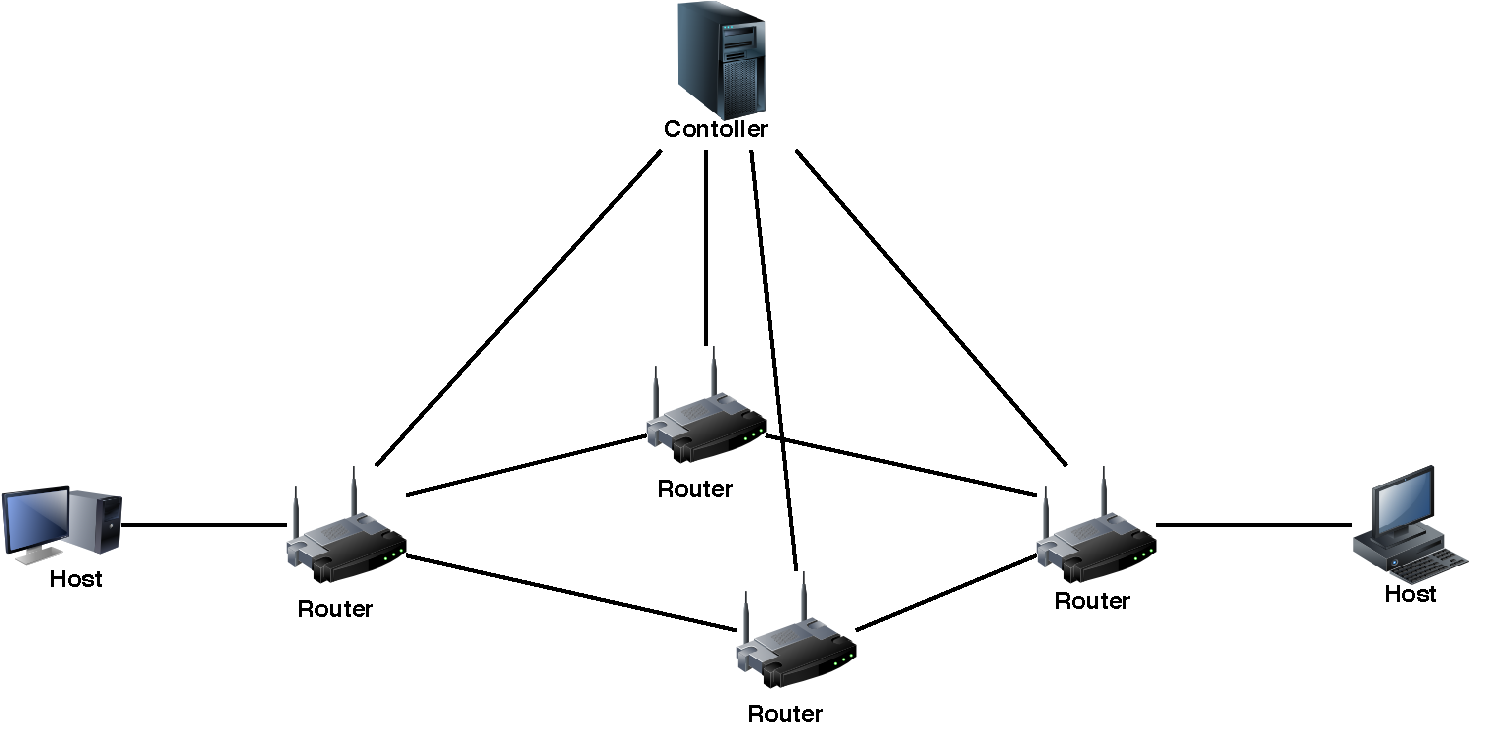
\includegraphics[scale = 0.60]{../images/psik_topology.pdf}
		\caption{Schemat architektury rozwiązania}
		\label{f:arch}
	\end{figure}	
	\section{Demonstracja rezultatów}
	W~ramach przedstawienia poprawności implementacji wyłączany będzie jeden z~routerów nie połączony z~hostem. Następnie zaprezentowany będzie przesył informacji z~jednego hosta do drugiego z~wykorzystaniem alternatywnej trasy. 
	\section{Cel częściowy}
	W~trakcie odbioru częściowego planowane jest pokazanie zaimplementowanej sieci, połączonej zgodnie z~rysunkiem \ref{f:arch}, w~której przesył danych pomiędzy hostami następuje po podstawowej ścieżce. 
	\section{Podział prac}
	Tabela \ref{t:podzial_prac} przedstawia ustalony podział pracy w~zespole.
	\begin{table}[h]
		\centering
		\begin{tabular}{|c|c|c|}
			%\begin{tabular}{|m{1.5em}|m{17 em}|m{16em}|}
			\hline
			osoba& Kamila Lis & Karolina Borkowska\\
			\hline
			zadania & implementacja sterownika& przygotowanie symulacji sieci\\
			\hline
		\end{tabular}	
		\caption{Podział prac w zespole}
		\label{t:podzial_prac}
	\end{table}
	
	

	
\end{document}